\documentclass[conference]{IEEEtran}
\IEEEoverridecommandlockouts
% The preceding line is only needed to identify funding in the first footnote. If that is unneeded, please comment it out.
\usepackage{cite}
\usepackage{amsmath,amssymb,amsfonts}
\usepackage{algorithmic}
\usepackage{graphicx}
\usepackage[utf8x]{inputenc} 
\usepackage{textcomp}
\usepackage{xcolor}
\usepackage{mathtools}

\def\BibTeX{{\rm B\kern-.05em{\sc i\kern-.025em b}\kern-.08em
    T\kern-.1667em\lower.7ex\hbox{E}\kern-.125emX}}
\begin{document}

\title{Understanding Image Advertisements and Predicting Sentiment\\}

\author{\IEEEauthorblockN{1\textsuperscript{st} Rohan Chopra}
\IEEEauthorblockA{\textit{40233019} \\
\textit{Concordia University}\\
Montreal, Canada \\
rohanchopra09@gmail.com}
\and
\IEEEauthorblockN{2\textsuperscript{nd} Harman Singh Jolly}
\IEEEauthorblockA{\textit{40204947} \\
\textit{Concordia University}\\
Montreal, Canada \\
jollyharmansingh@gmail.com}
}

\maketitle

\begin{abstract}
This document is a model and instructions for \LaTeX.
This and the IEEEtran.cls file define the components of your paper [title, text, heads, etc.]. *CRITICAL: Do Not Use Symbols, Special Characters, Footnotes, 
or Math in Paper Title or Abstract.
\end{abstract}

\begin{IEEEkeywords}
component, formatting, style, styling, insert
\end{IEEEkeywords}

\section{Introduction}
In this fast paced world, companies now trade with the ever changing data we generate. With data, comes along user profiling or a set of topics that a user can be defined into. Perhaps, the  expansion of online visual content and social media has led to a surge of interest in the investigation of large-scale social multimedia analysis. In recent years, image advertisements have become increasingly prevalent in our daily lives. From billboards to social media ads, companies are constantly vying for our attention through visually appealing images. However, with the rise of sentiment analysis, it is now possible to predict the emotions that these images evoke in viewers. So, pondering over the platitude, "A picture says a thousand words" becomes necessary.

Tech giants like Facebook and Google have produced enormous wealth by advertisements only where 97.5\% of the \$116.6 billion generated by Facebook \cite{b1} and 70.9\% of Google’s revenue \cite{b2} came in from broadcasting advertisements. Attracting customers to a product is a vital aspect of using  advertisements on both television and social media. Selection of ads by hand is a physically tedious and onerous job where provision of image based advertisements or videos becomes highly difficult via handpicking. So, automatic advertising techniques are developed, such as the contextual advertising method which aims to find the most relevant ad to a provided content without annoying customers.

The components that contribute to the effectiveness of these advertisements are intricate and are being analyzed in marketing science and consumer psychology. A particular focus of this research has been on comprehending the emotions and sentiments conveyed by visual media content, which has become increasingly popular for both academic and practical purposes. Sentiment analysis is a process of identifying and extracting opinions, emotions, and attitudes expressed in text. However, with the increasing use of visual media in advertising, there has been a need for sentiment analysis in images. Sentiment labels are used to annotate images with positive, negative or neutral sentiments. These annotations are used to train machine learning models to predict the emotions that an image is likely to evoke in viewers.
Powerful emotions conveyed by images and videos can amplify the message conveyed in the content, making it more impactful and capable of influencing the audience more effectively. But sometimes, advertisements aren’t able to hold viewers interest as the product shown doesn’t necessarily incline to the viewers choices or viewers actually skip watching advertisements that aren’t able to garner their attention, which is where a positive or a negative connotation comes into picture pertaining to sentiment of an advertisement.

Our report focuses on .


\section{Related Works}

% \subsection{Maintaining the Integrity of the Specifications}

In order to create an effective advertisement, researchers focus on tons of ideas to reach a balance of emotion and the type of message conveyed. The visual understanding or common sense that the “red color” symbolizes “stop” when used in traffic related series and symbolizes “blood” when used in medical related series is extremely potent in humans but negligible in computers. The recognition of non-photorealistic objects and symbolism are possible illustrations depicting the visual-rhetoric methods for conveying a message through ads. To fathom these rhetorics which not only requires the discernment of objects but also requires the decoding of this rhetoric \cite{b4} \cite{b5}. Perhaps, a summarization about the image can where it talks about \cite{b6} \cite{b7} which objects are portrayed, how they are portrayed and answering the primal questions as to why they are portrayed. For instance, if an advertisement is meant to target a young audience, it can be designed with bright colors and positive sentiments to appeal to that demographic. On the other hand, an ad meant for an older audience may be designed with muted colors and neutral sentiments. By predicting the sentiments that an advertisement is likely to evoke, companies can tailor their ads to specific audiences, increasing their chances of success.

Exploring objects or generic nouns such as “cat” or “trees” have been a marvel of machine vision but the association of sentiments correlating to the visuals remains a challenging and seemingly insurmountable task. The difficulty of this endeavor stems from the significant emotional distance between the low visual characteristics and the high-level sentiment that adjectives convey. To fill this gap between visual characteristics and sentiments, Borth, Damian et al. \cite{b8} proposed an alternative method that represents sentiment-related visual concepts for an intermediary  representation. They have coined the term Adjective Noun Pairs (ANP) like “sprawling trees” or “sleepy cat” which are used to corroborate the adjective of nouns, further used to identify nouns. Although ANPs do not directly express emotions or sentiments, they serve as useful statistical cues for detecting emotions conveyed in the images, as they were discovered based on strong co-occurrence relationships with emotion tags of web photos. In their study Borth, Damian et al \cite{b8} trained binary SVM classifiers on ANPs for whole images. To further enhance the classifiers, Chen, Felix et al. \cite{b9} incorporated object-based concept localization and the semantic similarity among the concepts. 

DeepSentiBank \cite{b10} hows significant efforts to interpret emotion from images using a model trained on web images that are tagged with multiple sentiments. Hussain, Zhang et al.
\cite{b11} went further to apply DeepSentiBank and reached a conclusion to observe a detector for natural images (DeepSentiBank) couldn’t be applicable for advertisement images. Besides DeepsentiBank, Vedula \& Sun et al. \cite{b12} developed an advertisement recommendation system using sentiments in multimedia content. Using deep learning techniques, image and video analysis combined have garnered a great amount of headway for data analysis at Youtube and for contextual understanding in video advertising \cite{b13}.
But, compared to other forms of media such as publishing or billboards, which are less personalized, a great deal of lacuna lies in interpreting advertisements media due to their extensive use of visual rhetoric as coined in Hussain, Zhang et al. \cite{b11}. 

An advertisement demands much in depth analysis due to the fact that they intend to persuade people for their motion by lobbying their product as best to make people aware of any social cause. Give an example of ad images here, some advertisement that represents a hidden social cause. The motive to persuade people is deeply imbibed inside an advertisement, where sometimes it is portrayed via simple tone or sometimes via sarcasm. In order to understand this underlying sentiment, only appearance isn’t enough. Therefore, to personalize the experience with ads, it is imperative to  not only understand its topic, but also the emotion it conveys. Zhang, Luo et al. \cite{b14} introduced a framework that amalgamates multiple modalities together for envisioning topic and sentiment related predictions to further conceptualize advertisements.

\section{Dataset}
Before you begin to format your paper, first write and save the content as a 
separate text file. Complete all content and organizational editing before 
formatting. Please note sections \ref{AA} below for more information on 
proofreading, spelling and grammar.

\begin{figure}[htbp]
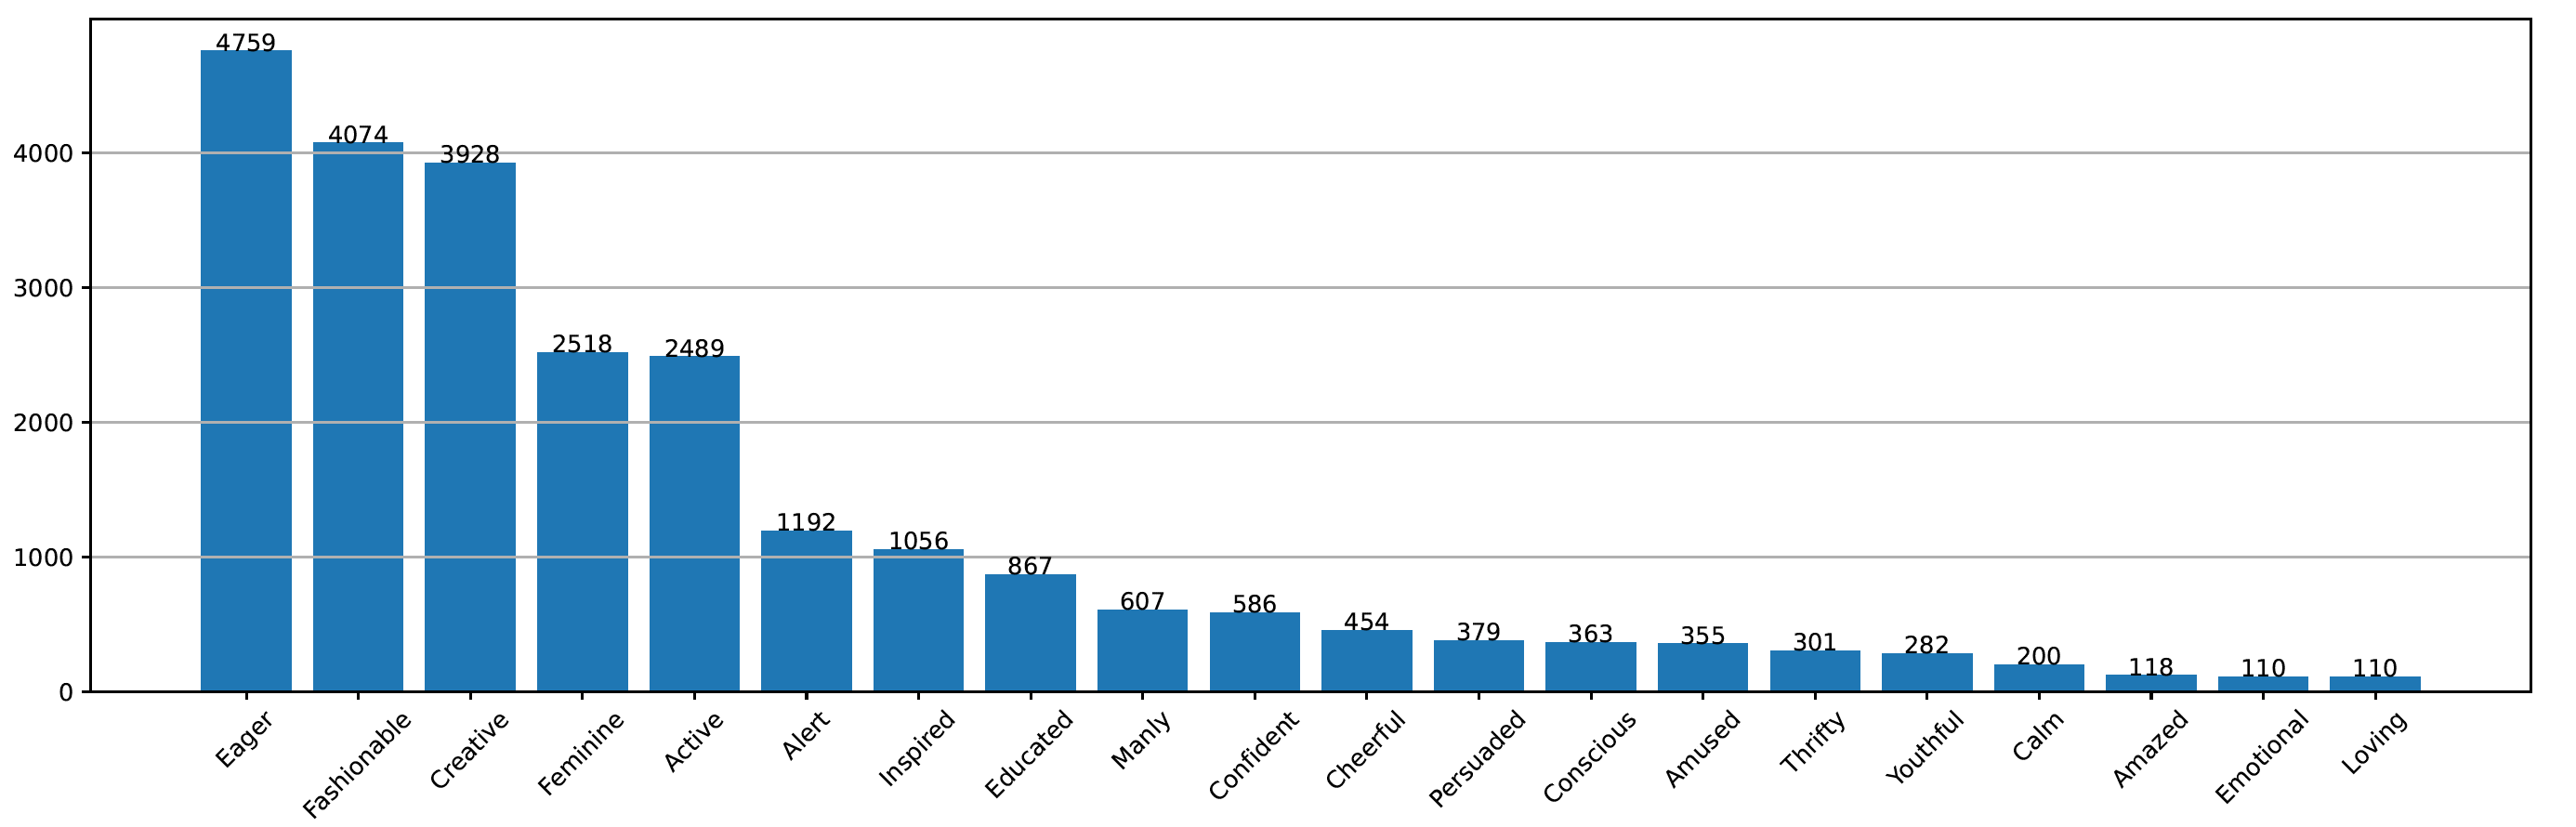
\includegraphics[width=9cm, height=10cm, keepaspectratio]{figures/dataset.eps}
\caption{Sentiment Label Distribution}
\label{fig}
\end{figure}

\section{Methodology}

Before training, the images have to processed for denoising and their quality improved before loading it to model for classification. 

\subsection{Bilateral Filter}
For improving the quality of the images, a bilateral filter was used. A smoothing filter for images, is used to reduce noise while preserving edges in a non-linear manner. This filter works by calculating a weighted average of intensity values from surrounding pixels to replace the intensity of each pixel. The weight of each pixel is determined using a Gaussian distribution and it preserves sharp edges. The weights used in the filter are not solely based on the distance between pixels, but also take into consideration differences in radiometric properties such as color intensity and depth distance \cite{b15}.

\begin{figure}[htp]
\includegraphics[width=9cm, height=11cm, keepaspectratio]{figures/ads_bilateral.eps}
\caption{Bilateral Filter applied on Ads }
\label{fig}
\end{figure}

As shown in fig 2, a bilateral filter is controlled by three parameters sigma(s), responsible for spatial region which smooths larger surfaces as we increase the spatial parameter, sigma(r) which tends to act like a Gaussian filter when it increases as the Gaussian range widens and d, which is the diameter of each pixel neighbourhood. It is quintessential to know that all other filters smudge the edges, while Bilateral Filtering retains them. When weights are multiplied together and if one of the weights is close to zero, no smoothing occurs. This can be demonstrated by using a large spatial Gaussian with a narrow range Gaussian, which results in limited smoothing despite the filter having a large spatial extent. The range weight ensures that the edges are preserved.

After applying different values d, sigma(s) and sigma(r), it was determined that the pixel diameter of 9 along with sigma(s) and sigma(r) being 9 as well gave the best results. Following that, bilateral filters have been applied twice merely because of the fact that applying bilateral filters in iterations enhanced picture quality even more. The image below depicts a significant change than the previous image i.e. the original image where the color banding or posterization, an ugly artifact that can be seen in digital images, has been notably reduced \cite{b16} and the final image is better than previous one. Another remarkable change was also witnessed which relates to compression artifacts, a distortion of media in images which is caused by lossy compression of media was removed  in the final image corroborating the efforts. 

\subsection{Pre-processing Techniques}
Pytorch provides various functional transformations that can be applied using the torchvision.transform module. They accept both PIL images and tensor images, although some transformations are PIL-only and some are tensor-only \cite{17}. As these transformations require a parameter such as a factor by which an image can be transformed, therefore they cannot be applied to all images owing to the factor that all images are different.

\begin{figure}[htbp]
    \includegraphics[width=9cm, height=9cm, keepaspectratio]{figures/preprocessing_plots.eps}
    \caption{Pytorch Preprocessing Techniques}
    \label{fig}
    \end{figure}

For example, a Hue transform that accepts an image along with a parameter, hue\_factor that ranges from [-0.5 to 0.5]. 0.5 and -0.5 give complete reversal of the hue channel in HSV space in positive and negative direction respectively whereas 0 means no shift. The same level factor cannot be expected from other techniques such as sharpness or contrast etc. Hence, this parameter cannot be kept constant for all images as it will have a variable effect or appeal on different images. In the fig below, five random images have been selected and functional image processing techniques like hue transforms, gamma transforms, solarize transformations, sharpness etc have been applied to reach a conclusion that all images bearing unique in their characteristics respond differently to functional transformations applied.

Even though brightness and contrast change show a potent outcome, a specific parameter cannot be kept for all images which points this approach to be handled in data augmentation where functions like AutoContrast and AutoBrightness have been applied. Histogram equalization, a popular technique for improving the contrast of the images visibly failed to work for colored images. This technique was employed on a colored image which visibly distorted colors and features such that it could not be considred as a viable pre-prcessing technique.

\begin{figure}[htbp] 
    \includegraphics[width=9cm, height=10cm, keepaspectratio]{figures/histogram_equalize.eps} 
    \caption{Histogram Equalization on Colored Image} 
    \label{fig} 
    \end{figure}

Some details about an image comparison between image 1 and image 2…..such that we are able to substantiate our findings.

\subsection{Data Augmentations Techniques}
Data augmentation plays a crucial role in completing the training requirements for deep learning models as these models aren’t able to converge the network to an optimal solution using some gradient based optimization algorithm. The huge number of parameters needed to be tuned by the learning algorithm require enormous amounts of data merely because of the fact that the deep learning algorithms start off with a poor initial state where weights are completely random. There are various ways to augment data using pytorch library such as RandomHorizontalFlip, RandomAdjustSharpness etc that produce images with any random factor for creating possible image outputs that may be a possible scenario in the real world for understanding the variability in the image dataset. 
In the images below, data augmentation has been visualized using RandomHorizontalFlip, RandomRotation to a certain degree, RandomAdjustSharpness with sharpness factor as 2,  RandomAutocontrast with factor as 5, and lastly RandomColorJitter.

\begin{figure}[htbp] 
    \includegraphics[width=9cm, height=10cm, keepaspectratio]{figures/RandomHorizontalFlip.eps} 
    \caption{Data Augmentation using RandomHorizontalFlip} 
    \label{fig} 
    \end{figure}

\begin{figure}[htbp] 
    \includegraphics[width=9cm, height=10cm, keepaspectratio]{figures/RandomRotation30.eps} 
    \caption{Data Augmentation using RandomRotation at 30 degrees} 
    \label{fig} 
    \end{figure}

\begin{figure}[htbp] 
    \includegraphics[width=9cm, height=10cm, keepaspectratio]{figures/RandomAdjustSharpness.eps} 
    \caption{Data Augmentation using RandomAdjustSharpness} 
    \label{fig} 
    \end{figure}

\begin{figure}[htbp] 
    \includegraphics[width=9cm, height=10cm, keepaspectratio]{figures/RandomAutocontrast.eps} 
    \caption{Data Augmentation using RandomAutocontrast} 
    \label{fig} 
    \end{figure}

\begin{figure}[htbp] 
    \includegraphics[width=9cm, height=10cm, keepaspectratio]{figures/ColorJitter.eps} 
    \caption{Data Augmentation using ColorJitter} 
    \label{fig} 
    \end{figure}

\begin{thebibliography}{00}
\bibitem{b1} https://www.oberlo.com/statistics/facebook-ad-revenue

\bibitem{b2} https://www.statista.com/statistics/266249/advertising-revenue-of-google/

\bibitem{b3} Mei, Tao, Xian-Sheng Hua, Linjun Yang, and Shipeng Li. "VideoSense: towards effective online video advertising." In Proceedings of the 15th ACM international conference on Multimedia, pp. 1075-1084. 2007.

\bibitem{b4} Girshick, Ross. "Fast r-cnn." In Proceedings of the IEEE international conference on computer vision, pp. 1440-1448. 2015.

\bibitem{b5} Szegedy, Christian, Wei Liu, Yangqing Jia, Pierre Sermanet, Scott Reed, Dragomir Anguelov, Dumitru Erhan, Vincent Vanhoucke, and Andrew Rabinovich. "Going deeper with convolutions." In Proceedings of the IEEE conference on computer vision and pattern recognition, pp. 1-9. 2015.

\bibitem{b6} Y. Donahue, Jeffrey, Lisa Anne Hendricks, Sergio Guadarrama, Marcus Rohrbach, Subhashini Venugopalan, Kate Saenko, and Trevor Darrell. "Long-term recurrent convolutional networks for visual recognition and description." In Proceedings of the IEEE conference on computer vision and pattern recognition, pp. 2625-2634. 2015.

\bibitem{b7} Vinyals, Oriol, Alexander Toshev, Samy Bengio, and Dumitru Erhan. "Show and tell: A neural image caption generator." In Proceedings of the IEEE conference on computer vision and pattern recognition, pp. 3156-3164. 2015.

\bibitem{b8} Borth, Damian, Rongrong Ji, Tao Chen, Thomas Breuel, and Shih-Fu Chang. "Large-scale visual sentiment ontology and detectors using adjective noun pairs." In Proceedings of the 21st ACM international conference on Multimedia, pp. 223-232. 2013.

\bibitem{b9} Chen, Tao, Felix X. Yu, Jiawei Chen, Yin Cui, Yan-Ying Chen, and Shih-Fu Chang. "Object-based visual sentiment concept analysis and application." In Proceedings of the 22nd ACM international conference on Multimedia, pp. 367-376. 2014.

\bibitem{b10} Chen, Tao, Damian Borth, Trevor Darrell, and Shih-Fu Chang. "Deepsentibank: Visual sentiment concept classification with deep convolutional neural networks." arXiv preprint arXiv:1410.8586 (2014).

\bibitem{b11} Hussain, Zaeem, Mingda Zhang, Xiaozhong Zhang, Keren Ye, Christopher Thomas, Zuha Agha, Nathan Ong, and Adriana Kovashka. "Automatic understanding of image and video advertisements." In Proceedings of the IEEE conference on computer vision and pattern recognition, pp. 1705-1715. 2017.

\bibitem{b12} Vedula, Nikhita, Wei Sun, Hyunhwan Lee, Harsh Gupta, Mitsunori Ogihara, Joseph Johnson, Gang Ren, and Srinivasan Parthasarathy. "Multimodal content analysis for effective advertisements on youtube." In 2017 IEEE international conference on data mining (ICDM), pp. 1123-1128. IEEE, 2017.

\bibitem{b13} Madhok, Rishi, Shashank Mujumdar, Nitin Gupta, and Sameep Mehta. "Semantic understanding for contextual in-video advertising." In Proceedings of the AAAI Conference on Artificial Intelligence, vol. 32, no. 1. 2018.

\bibitem{b14} Zhang, Huaizheng, Yong Luo, Qiming Ai, Yonggang Wen, and Han Hu. "Look, read and feel: Benchmarking ads understanding with multimodal multitask learning." In Proceedings of the 28th ACM International Conference on Multimedia, pp. 430-438. 2020.

\bibitem{b15} https://en.wikipedia.org/wiki/Bilateral\_filter

\bibitem{b16} https://www.willgibbons.com/color-banding/

\bibitem{b17} https://pytorch.org/vision/stable/transforms.html

\end{thebibliography}
\vspace{12pt}
\color{red}
IEEE conference templates contain guidance text for composing and formatting conference papers. Please ensure that all template text is removed from your conference paper prior to submission to the conference. Failure to remove the template text from your paper may result in your paper not being published.

\end{document}
